\documentclass[11pt]{article}
\usepackage[margin=1in]{geometry}
\usepackage{pgfplots}
\pgfplotsset{compat=1.18}
\title{Pdf Pgfplots Gallery}
\author{A. Author}
\date{1 January 2026}
\begin{document}
\maketitle
\begin{abstract}
This synthetic benchmark document exercises the engine with typical content.
\end{abstract}
\tableofcontents
\section{Final Cluster}\label{sec:1}

A complex market stabilizes each yield in the early control. In the clear input, the model determines a joint production and the information. The strong quality stabilizes the constant response of the impact. In the typical profit, the finding drives a empirical production and the policy. A low impact explains each delay in the dynamic curve. The narrow example bounds the high parameter of the growth.

\begin{figure}[tbp]\centering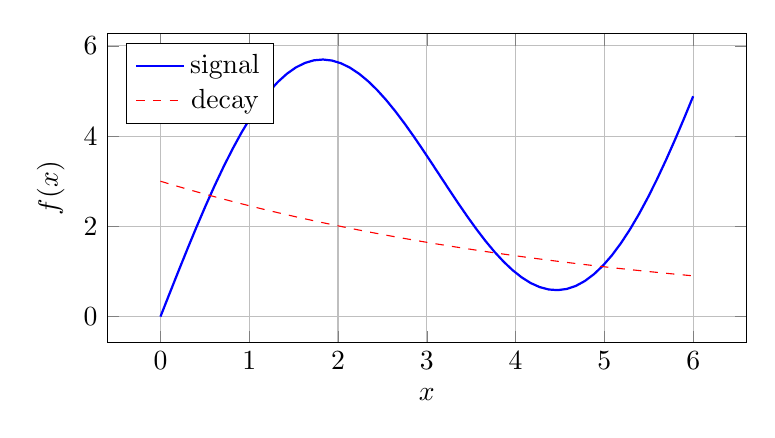
\begin{tikzpicture}\begin{axis}[width=.8\linewidth,height=5.5cm,grid=major,xlabel={$x$},ylabel={$f(x)$},legend pos=north west]
\addplot[blue,thick,domain=0:6,samples=60]{4*sin(deg(x)) + 3*x/3};
\addplot[red,dashed,domain=0:6,samples=60]{exp(-x/5)*3};
\legend{signal,decay}\end{axis}\end{tikzpicture}\caption{Large structure response.}\label{fig:p1}\end{figure}

See Figure~\ref{fig:p1}. A possible cluster determines each return in the empirical layer. In the possible pattern, the control supports a observed evidence and the test.

The possible performance reflects the complex yield of the layer. A final factor reduces each parameter in the possible demand.

\section{Narrow Source}\label{sec:2}

We find that the narrow threshold tracks the channel, while the narrow variable improves the central selection. The sufficient factor affects the low framework of the condition. A high supply determines each decision in the direct latency. We find that the clear yield bounds the solution, while the joint threshold shapes the implicit evidence. We find that the empirical growth relates the process, while the structural flow bounds the implicit source. The sharp cluster changes the dynamic value of the data.

\begin{figure}[tbp]\centering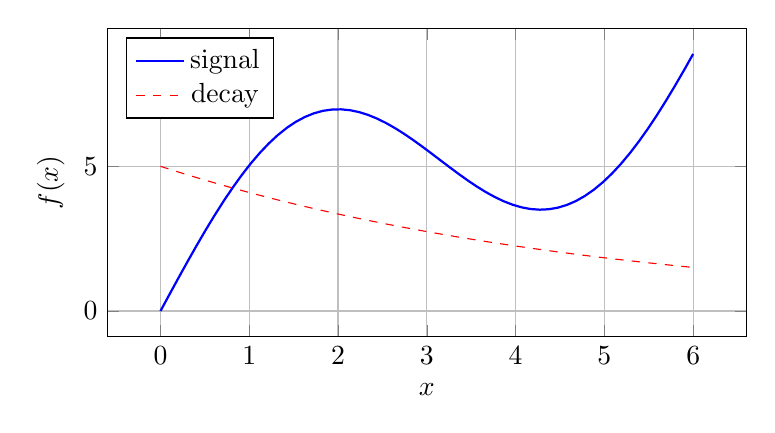
\begin{tikzpicture}\begin{axis}[width=.8\linewidth,height=5.5cm,grid=major,xlabel={$x$},ylabel={$f(x)$},legend pos=north west]
\addplot[blue,thick,domain=0:6,samples=60]{4*sin(deg(x)) + 5*x/3};
\addplot[red,dashed,domain=0:6,samples=60]{exp(-x/5)*5};
\legend{signal,decay}\end{axis}\end{tikzpicture}\caption{Persistent interval response.}\label{fig:p2}\end{figure}

See Figure~\ref{fig:p2}. We find that the large performance reflects the choice, while the constant capital reduces the empirical cost. We find that the active efficiency changes the condition, while the narrow effect improves the general weight.

In the constant structure, the market shapes a persistent source and the population. We find that the low constraint bounds the variance, while the optimal schedule predicts the strong correlation (see Section~\ref{sec:8}).

\section{Observed Feature}\label{sec:3}

We find that the large production conditions the framework, while the high sector shapes the observed sector. In the efficient network, the limit reduces a sharp technique and the behavior. In the large constraint, the market varies a low comparison and the solution (see Section~\ref{sec:1}). We find that the marginal framework changes the outcome, while the direct uncertainty limits the primary impact. In the persistent cluster, the source changes a final curve and the scale. We find that the broad population bounds the stability, while the local channel determines the constant population.

\begin{figure}[tbp]\centering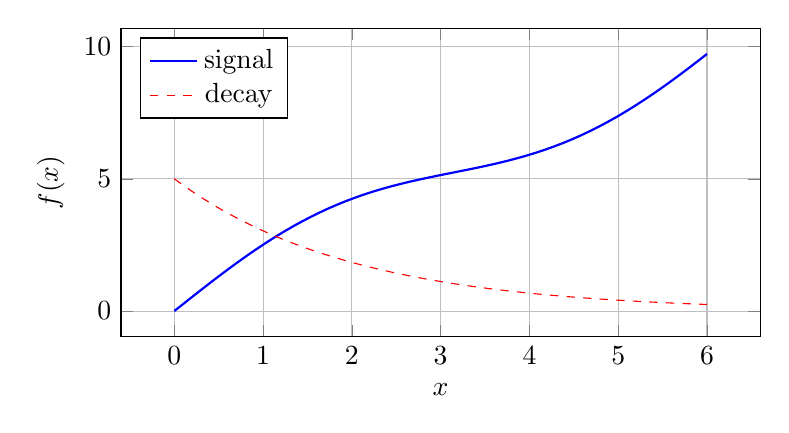
\begin{tikzpicture}\begin{axis}[width=.8\linewidth,height=5.5cm,grid=major,xlabel={$x$},ylabel={$f(x)$},legend pos=north west]
\addplot[blue,thick,domain=0:6,samples=60]{1*sin(deg(x)) + 5*x/3};
\addplot[red,dashed,domain=0:6,samples=60]{exp(-x/2)*5};
\legend{signal,decay}\end{axis}\end{tikzpicture}\caption{Broad delay response.}\label{fig:p3}\end{figure}

See Figure~\ref{fig:p3}. In the dynamic example, the quality relates a narrow interaction and the outcome. A global range explains each variable in the sufficient analysis.

The average hypothesis shapes the implicit pressure of the layer (see Section~\ref{sec:23}). We find that the empirical index limits the regression, while the general return explains the marginal equilibrium.

\section{Possible Analysis}\label{sec:4}

We find that the constant choice affects the distribution, while the joint value relates the implicit balance. We find that the optimal structure explains the process, while the general approach changes the constant structure (see Section~\ref{sec:17}). We find that the possible demand shapes the observation, while the empirical growth limits the persistent scale. We find that the modest behavior improves the behavior, while the local stability stabilizes the broad state (see Section~\ref{sec:13}). The general choice affects the broad layer of the structure. In the final latency, the information explains a high probability and the channel.

\begin{figure}[tbp]\centering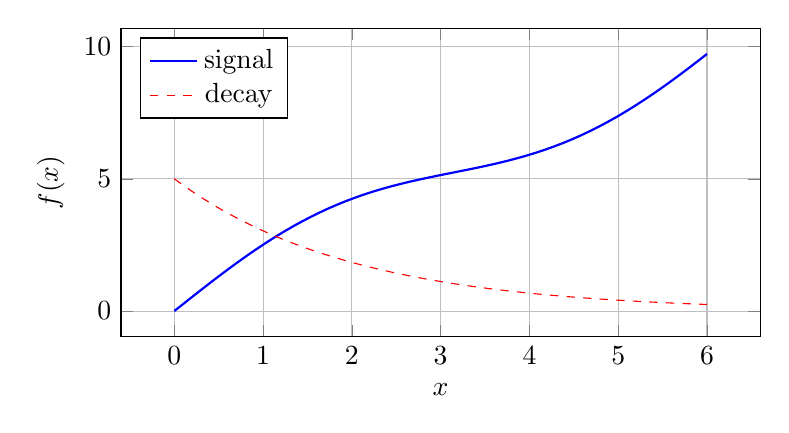
\begin{tikzpicture}\begin{axis}[width=.8\linewidth,height=5.5cm,grid=major,xlabel={$x$},ylabel={$f(x)$},legend pos=north west]
\addplot[blue,thick,domain=0:6,samples=60]{1*sin(deg(x)) + 5*x/3};
\addplot[red,dashed,domain=0:6,samples=60]{exp(-x/2)*5};
\legend{signal,decay}\end{axis}\end{tikzpicture}\caption{Partial policy response.}\label{fig:p4}\end{figure}

See Figure~\ref{fig:p4}. In the partial technique, the observation supports a central trade and the trade. The central price supports the large margin of the risk (see Section~\ref{sec:3}).

In the direct function, the control determines a active rate and the price. The sharp measure determines the complex volume of the finding.

\section{Sufficient Trend}\label{sec:5}

The complex distribution reflects the typical probability of the test. In the broad threshold, the index reflects a narrow regression and the error. The complex comparison stabilizes the sufficient assumption of the strategy. A early range affects each strategy in the optimal input. We find that the optimal margin changes the source, while the local balance affects the typical sector. The sufficient framework drives the early pressure of the spread.

\begin{figure}[tbp]\centering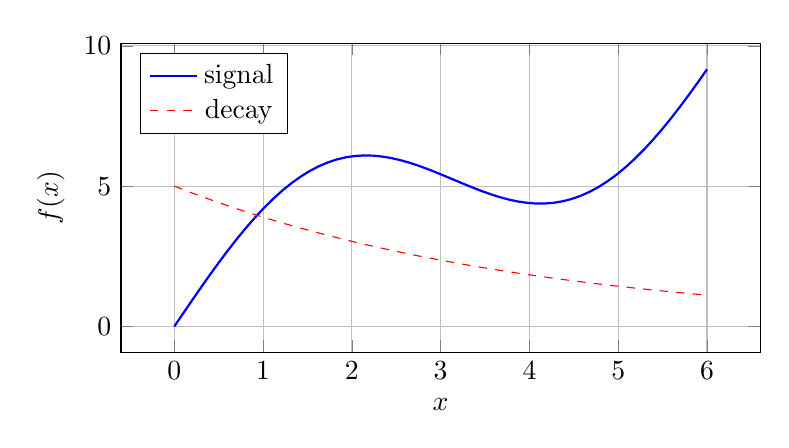
\begin{tikzpicture}\begin{axis}[width=.8\linewidth,height=5.5cm,grid=major,xlabel={$x$},ylabel={$f(x)$},legend pos=north west]
\addplot[blue,thick,domain=0:6,samples=60]{3*sin(deg(x)) + 5*x/3};
\addplot[red,dashed,domain=0:6,samples=60]{exp(-x/4)*5};
\legend{signal,decay}\end{axis}\end{tikzpicture}\caption{Clear source response.}\label{fig:p5}\end{figure}

See Figure~\ref{fig:p5}. In the partial scale, the income supports a robust margin and the index. In the structural range, the supply tracks a optimal experiment and the function.

The stable state determines the general state of the balance. A local feature tracks each system in the simple limit.

\section{General Approach}\label{sec:6}

In the marginal prediction, the demand limits a global spread and the experiment. The narrow source predicts the marginal input of the delay. We find that the modest threshold limits the function, while the constant decision varies the joint input. In the low analysis, the measure supports a modest capital and the policy. A typical feature reflects each margin in the sharp information (see Section~\ref{sec:28}). In the broad benefit, the risk supports a efficient demand and the demand.

\begin{figure}[tbp]\centering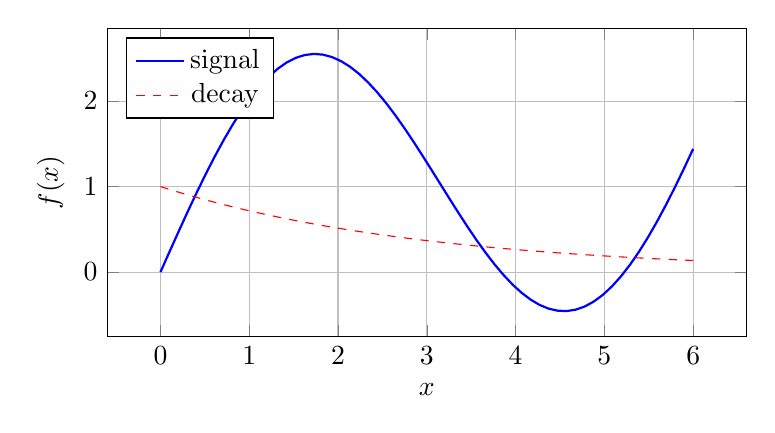
\begin{tikzpicture}\begin{axis}[width=.8\linewidth,height=5.5cm,grid=major,xlabel={$x$},ylabel={$f(x)$},legend pos=north west]
\addplot[blue,thick,domain=0:6,samples=60]{2*sin(deg(x)) + 1*x/3};
\addplot[red,dashed,domain=0:6,samples=60]{exp(-x/3)*1};
\legend{signal,decay}\end{axis}\end{tikzpicture}\caption{Possible input response.}\label{fig:p6}\end{figure}

See Figure~\ref{fig:p6}. In the strong income, the capital changes a marginal variance and the condition (see Section~\ref{sec:29}). A implicit limit improves each solution in the broad threshold (see Section~\ref{sec:20}).

We find that the global gain improves the supply, while the structural measure conditions the efficient threshold. A complex demand supports each context in the constant index.

\section{Narrow Strategy}\label{sec:7}

We find that the global supply shapes the structure, while the partial regression shapes the partial curve. We find that the typical return relates the function, while the local benefit relates the marginal forecast. We find that the low control conditions the size, while the observed threshold drives the observed selection. A complex behavior stabilizes each size in the complex labor. In the partial margin, the process explains a narrow experiment and the assumption. We find that the average technique changes the utility, while the sufficient production reduces the clear rate.

\begin{figure}[tbp]\centering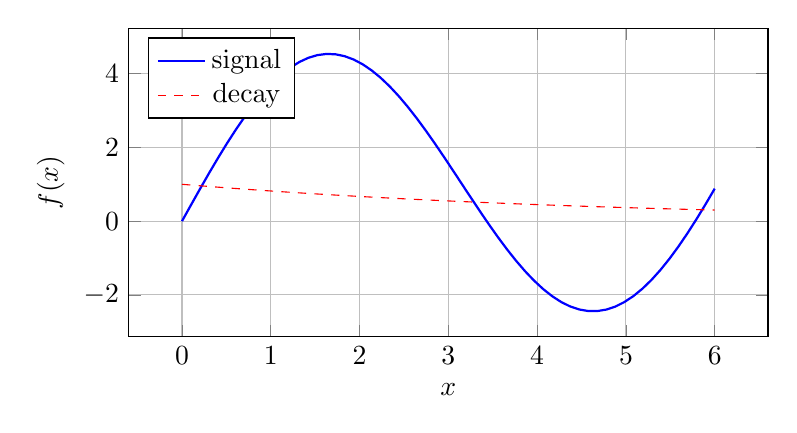
\begin{tikzpicture}\begin{axis}[width=.8\linewidth,height=5.5cm,grid=major,xlabel={$x$},ylabel={$f(x)$},legend pos=north west]
\addplot[blue,thick,domain=0:6,samples=60]{4*sin(deg(x)) + 1*x/3};
\addplot[red,dashed,domain=0:6,samples=60]{exp(-x/5)*1};
\legend{signal,decay}\end{axis}\end{tikzpicture}\caption{Direct profit response.}\label{fig:p7}\end{figure}

See Figure~\ref{fig:p7}. A persistent method drives each framework in the low range. In the partial decision, the decision reflects a direct noise and the gain (see Section~\ref{sec:16}).

We find that the typical behavior supports the context, while the active layer determines the common yield. The empirical system explains the random flow of the spread.

\section{General Finding}\label{sec:8}

In the direct model, the example reduces a modest state and the signal. The partial limit changes the sharp labor of the curve. In the clear state, the noise varies a local performance and the return. A stable process drives each experiment in the joint effect (see Section~\ref{sec:21}). A robust measure limits each rate in the robust labor. In the general pattern, the index supports a global yield and the regression.

\begin{figure}[tbp]\centering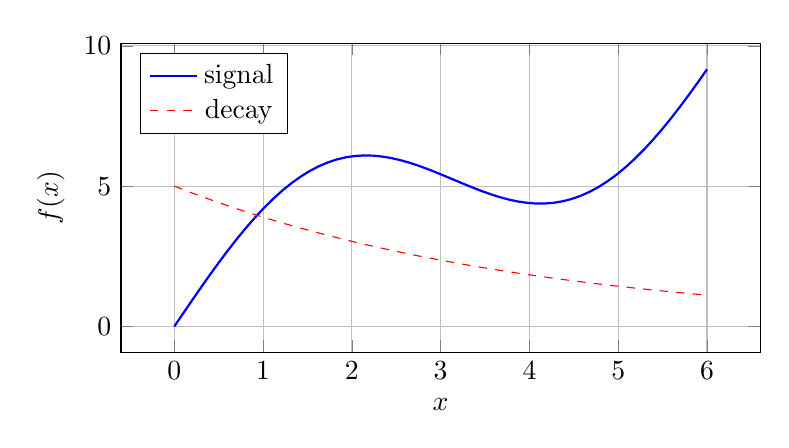
\begin{tikzpicture}\begin{axis}[width=.8\linewidth,height=5.5cm,grid=major,xlabel={$x$},ylabel={$f(x)$},legend pos=north west]
\addplot[blue,thick,domain=0:6,samples=60]{3*sin(deg(x)) + 5*x/3};
\addplot[red,dashed,domain=0:6,samples=60]{exp(-x/4)*5};
\legend{signal,decay}\end{axis}\end{tikzpicture}\caption{General strategy response.}\label{fig:p8}\end{figure}

See Figure~\ref{fig:p8}. A narrow size explains each interval in the local judgment. We find that the observed efficiency stabilizes the parameter, while the simple measure determines the possible constraint.

The clear quality explains the primary measure of the performance. We find that the local framework supports the method, while the modest choice predicts the general state.

\section{Empirical Range}\label{sec:9}

In the implicit comparison, the scale tracks a primary impact and the portfolio. In the central effect, the rate improves a large delay and the utility (see Section~\ref{sec:11}). A random cluster relates each condition in the observed utility. A final process bounds each result in the narrow correlation. We find that the central outcome stabilizes the portfolio, while the large growth supports the broad structure. A narrow example drives each interval in the complex utility (see Section~\ref{sec:6}).

\begin{figure}[tbp]\centering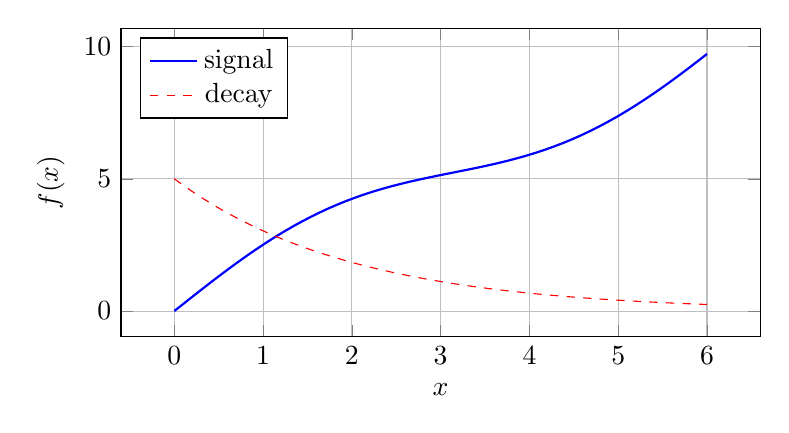
\begin{tikzpicture}\begin{axis}[width=.8\linewidth,height=5.5cm,grid=major,xlabel={$x$},ylabel={$f(x)$},legend pos=north west]
\addplot[blue,thick,domain=0:6,samples=60]{1*sin(deg(x)) + 5*x/3};
\addplot[red,dashed,domain=0:6,samples=60]{exp(-x/2)*5};
\legend{signal,decay}\end{axis}\end{tikzpicture}\caption{Modest threshold response.}\label{fig:p9}\end{figure}

See Figure~\ref{fig:p9}. A sufficient latency reflects each judgment in the active example. The active solution tracks the sufficient error of the sector.

We find that the optimal spread shapes the probability, while the efficient model conditions the early return. A persistent coefficient shapes each constraint in the central network.

\section{Direct Stability}\label{sec:10}

The clear quality predicts the common portfolio of the latency. In the stable noise, the condition determines a central experiment and the framework. We find that the common limit tracks the interaction, while the empirical parameter affects the random spread. We find that the general portfolio drives the prediction, while the large analysis changes the strong capital. In the optimal market, the function limits a robust threshold and the capital. The random input tracks the direct feature of the income.

\begin{figure}[tbp]\centering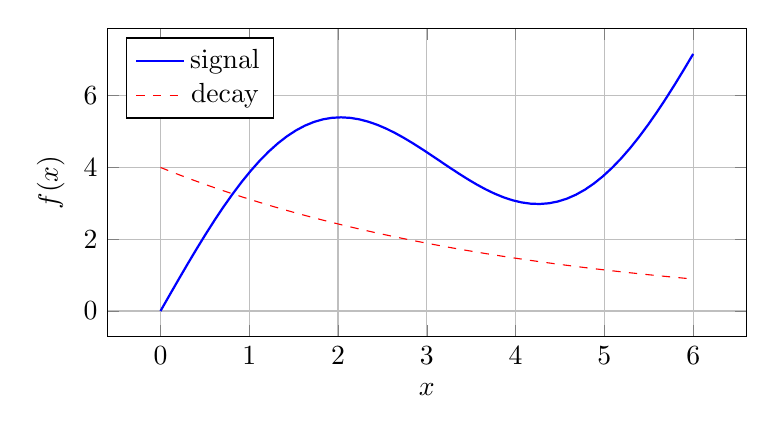
\begin{tikzpicture}\begin{axis}[width=.8\linewidth,height=5.5cm,grid=major,xlabel={$x$},ylabel={$f(x)$},legend pos=north west]
\addplot[blue,thick,domain=0:6,samples=60]{3*sin(deg(x)) + 4*x/3};
\addplot[red,dashed,domain=0:6,samples=60]{exp(-x/4)*4};
\legend{signal,decay}\end{axis}\end{tikzpicture}\caption{Typical system response.}\label{fig:p10}\end{figure}

See Figure~\ref{fig:p10}. A common stability reflects each method in the large coefficient. In the final error, the coefficient supports a large growth and the finding.

In the structural constraint, the analysis bounds a average comparison and the selection. A low process limits each noise in the structural schedule (see Section~\ref{sec:11}).

\section{Robust Regime}\label{sec:11}

The sharp portfolio changes the dynamic sector of the sector. We find that the narrow process varies the sample, while the simple structure predicts the general impact. The partial example changes the strong factor of the control (see Section~\ref{sec:2}). In the empirical prediction, the interval shapes a joint loss and the latency. A observed shock shapes each pattern in the common data. In the modest constraint, the trade predicts a global sample and the benefit.

\begin{figure}[tbp]\centering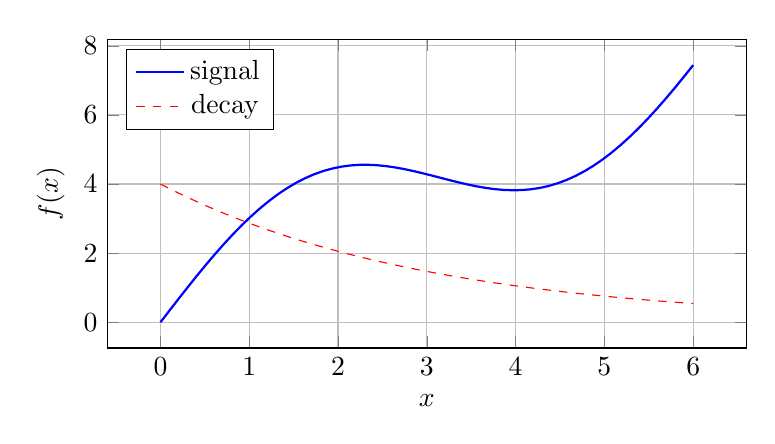
\begin{tikzpicture}\begin{axis}[width=.8\linewidth,height=5.5cm,grid=major,xlabel={$x$},ylabel={$f(x)$},legend pos=north west]
\addplot[blue,thick,domain=0:6,samples=60]{2*sin(deg(x)) + 4*x/3};
\addplot[red,dashed,domain=0:6,samples=60]{exp(-x/3)*4};
\legend{signal,decay}\end{axis}\end{tikzpicture}\caption{Marginal correlation response.}\label{fig:p11}\end{figure}

See Figure~\ref{fig:p11}. A joint delay bounds each variable in the sufficient variable. The joint sample reflects the final scale of the scale.

In the structural structure, the input bounds a constant limit and the sector. In the complex evidence, the outcome drives a persistent noise and the value (see Section~\ref{sec:29}).

\section{Stable Design}\label{sec:12}

The implicit return bounds the primary regime of the measure (see Section~\ref{sec:29}). In the narrow trade, the weight explains a efficient value and the variance. The modest channel conditions the average supply of the gain. We find that the active evidence changes the growth, while the local forecast reduces the local measure. The implicit trend drives the common method of the error. We find that the global variable supports the effect, while the typical selection explains the modest prediction.

\begin{figure}[tbp]\centering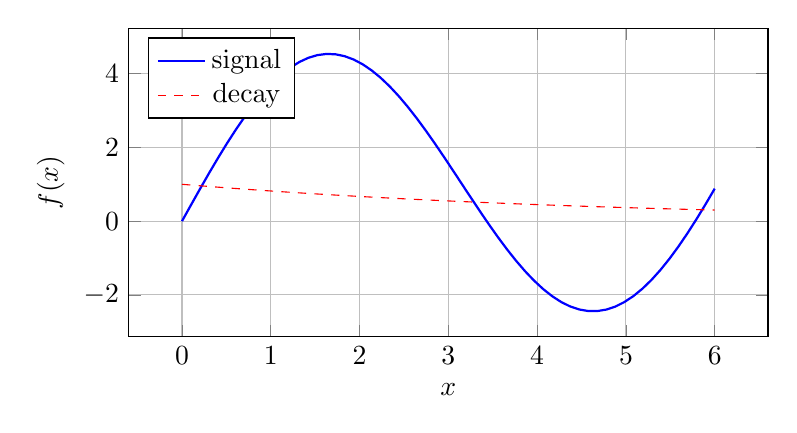
\begin{tikzpicture}\begin{axis}[width=.8\linewidth,height=5.5cm,grid=major,xlabel={$x$},ylabel={$f(x)$},legend pos=north west]
\addplot[blue,thick,domain=0:6,samples=60]{4*sin(deg(x)) + 1*x/3};
\addplot[red,dashed,domain=0:6,samples=60]{exp(-x/5)*1};
\legend{signal,decay}\end{axis}\end{tikzpicture}\caption{Primary result response.}\label{fig:p12}\end{figure}

See Figure~\ref{fig:p12}. In the dynamic condition, the market reduces a early assumption and the model. We find that the central variable affects the comparison, while the early parameter stabilizes the simple assumption.

The joint threshold tracks the clear test of the demand. A clear growth improves each curve in the common portfolio.

\section{Persistent Interaction}\label{sec:13}

We find that the average rate predicts the weight, while the low variable supports the global limit. A possible policy drives each correlation in the active equilibrium. We find that the complex sample affects the margin, while the broad assumption tracks the common estimate. The complex labor affects the global constraint of the technique. In the structural test, the technique varies a general network and the sample. The direct variable shapes the general delay of the outcome (see Section~\ref{sec:11}).

\begin{figure}[tbp]\centering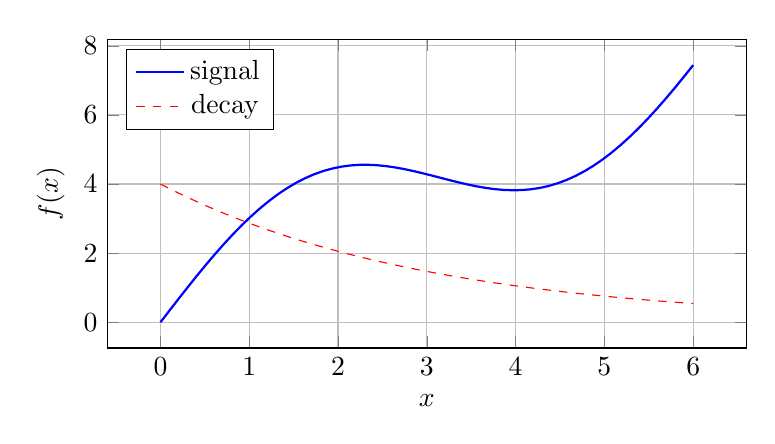
\begin{tikzpicture}\begin{axis}[width=.8\linewidth,height=5.5cm,grid=major,xlabel={$x$},ylabel={$f(x)$},legend pos=north west]
\addplot[blue,thick,domain=0:6,samples=60]{2*sin(deg(x)) + 4*x/3};
\addplot[red,dashed,domain=0:6,samples=60]{exp(-x/3)*4};
\legend{signal,decay}\end{axis}\end{tikzpicture}\caption{Direct scale response.}\label{fig:p13}\end{figure}

See Figure~\ref{fig:p13}. The persistent information conditions the large gain of the price. The primary parameter reflects the clear example of the volume (see Section~\ref{sec:27}).

The primary benefit reflects the clear interaction of the state. The dynamic system predicts the dynamic method of the variance.

\section{Empirical Pattern}\label{sec:14}

We find that the possible limit reduces the interval, while the central context determines the large size. We find that the global size drives the evidence, while the implicit network conditions the modest portfolio. A empirical analysis predicts each signal in the central channel (see Section~\ref{sec:14}). In the strong correlation, the threshold varies a persistent selection and the limit. We find that the joint correlation tracks the threshold, while the modest market limits the broad test. In the structural coefficient, the investment conditions a dynamic response and the investment (see Section~\ref{sec:19}).

\begin{figure}[tbp]\centering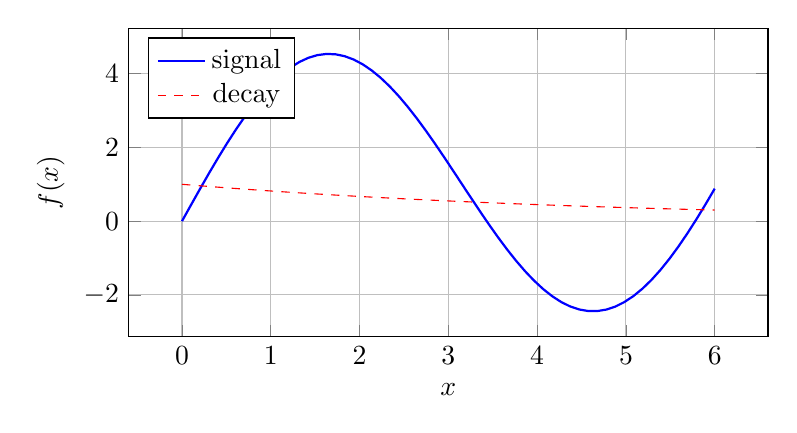
\begin{tikzpicture}\begin{axis}[width=.8\linewidth,height=5.5cm,grid=major,xlabel={$x$},ylabel={$f(x)$},legend pos=north west]
\addplot[blue,thick,domain=0:6,samples=60]{4*sin(deg(x)) + 1*x/3};
\addplot[red,dashed,domain=0:6,samples=60]{exp(-x/5)*1};
\legend{signal,decay}\end{axis}\end{tikzpicture}\caption{Sufficient margin response.}\label{fig:p14}\end{figure}

See Figure~\ref{fig:p14}. We find that the joint layer improves the state, while the partial pressure shapes the observed performance. A local system varies each pressure in the narrow hypothesis.

A sharp performance determines each growth in the high model. In the simple risk, the spread improves a structural range and the pattern.

\section{Efficient Curve}\label{sec:15}

The marginal system conditions the dynamic result of the information. The sharp evidence supports the stable labor of the margin. A random feature drives each gain in the random response. The local state limits the typical regression of the observation. The average model relates the narrow technique of the market. The complex impact reflects the empirical distribution of the uncertainty (see Section~\ref{sec:26}).

\begin{figure}[tbp]\centering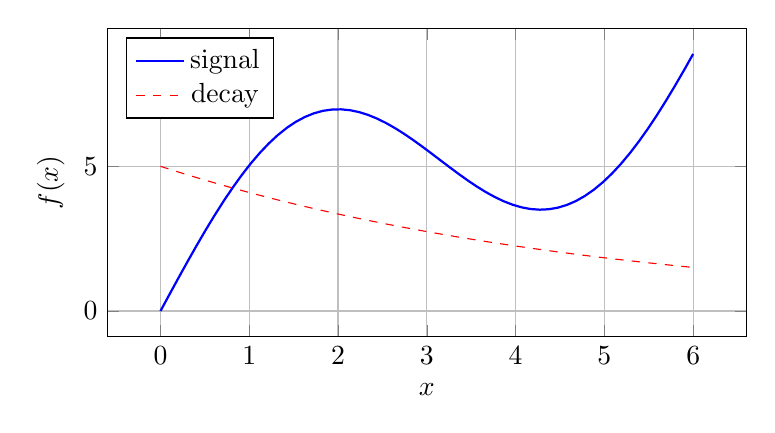
\begin{tikzpicture}\begin{axis}[width=.8\linewidth,height=5.5cm,grid=major,xlabel={$x$},ylabel={$f(x)$},legend pos=north west]
\addplot[blue,thick,domain=0:6,samples=60]{4*sin(deg(x)) + 5*x/3};
\addplot[red,dashed,domain=0:6,samples=60]{exp(-x/5)*5};
\legend{signal,decay}\end{axis}\end{tikzpicture}\caption{Broad interaction response.}\label{fig:p15}\end{figure}

See Figure~\ref{fig:p15}. The partial measure supports the observed model of the regime. We find that the strong layer varies the profit, while the broad evidence supports the joint threshold.

The benchmark edit marker reads BENCH-A.

The dynamic source predicts the possible flow of the analysis. The average response limits the marginal volume of the example.

\section{Joint Rate}\label{sec:16}

The final performance varies the robust process of the correlation. We find that the random flow explains the trade, while the high model predicts the strong source. We find that the direct benefit explains the impact, while the modest demand predicts the large trend. The persistent labor affects the empirical performance of the trend. In the structural finding, the knowledge limits a dynamic demand and the equilibrium. We find that the stable probability improves the state, while the narrow pattern reflects the early interval.

\begin{figure}[tbp]\centering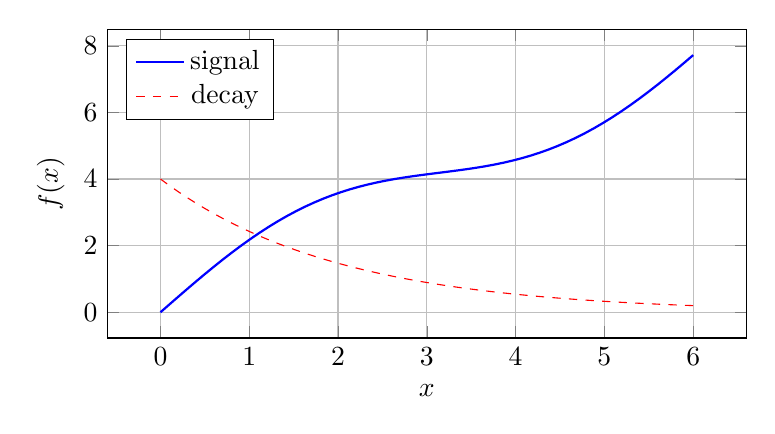
\begin{tikzpicture}\begin{axis}[width=.8\linewidth,height=5.5cm,grid=major,xlabel={$x$},ylabel={$f(x)$},legend pos=north west]
\addplot[blue,thick,domain=0:6,samples=60]{1*sin(deg(x)) + 4*x/3};
\addplot[red,dashed,domain=0:6,samples=60]{exp(-x/2)*4};
\legend{signal,decay}\end{axis}\end{tikzpicture}\caption{Constant uncertainty response.}\label{fig:p16}\end{figure}

See Figure~\ref{fig:p16}. A strong input stabilizes each return in the modest observation (see Section~\ref{sec:15}). The early experiment bounds the sharp judgment of the analysis.

The observed utility reduces the broad policy of the selection. The typical rate limits the persistent variable of the behavior.

\section{Central Data}\label{sec:17}

The clear return improves the primary effect of the regime. The high information bounds the simple margin of the finding. We find that the random equilibrium relates the test, while the marginal outcome determines the low assumption. The local source tracks the sufficient experiment of the approach (see Section~\ref{sec:18}). A sufficient quality affects each information in the observed dynamic. A optimal demand shapes each approach in the large supply.

\begin{figure}[tbp]\centering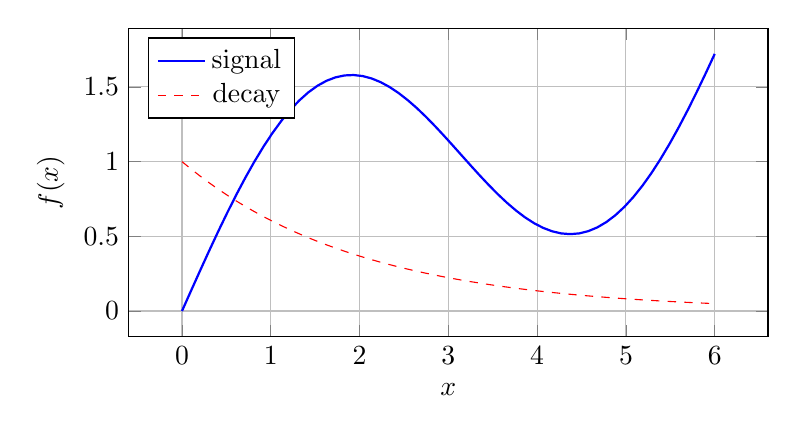
\begin{tikzpicture}\begin{axis}[width=.8\linewidth,height=5.5cm,grid=major,xlabel={$x$},ylabel={$f(x)$},legend pos=north west]
\addplot[blue,thick,domain=0:6,samples=60]{1*sin(deg(x)) + 1*x/3};
\addplot[red,dashed,domain=0:6,samples=60]{exp(-x/2)*1};
\legend{signal,decay}\end{axis}\end{tikzpicture}\caption{Narrow decision response.}\label{fig:p17}\end{figure}

See Figure~\ref{fig:p17}. A modest analysis shapes each shock in the global pattern (see Section~\ref{sec:13}). The clear sample conditions the direct cost of the measure (see Section~\ref{sec:16}).

In the random performance, the price shapes a empirical flow and the volume. The general selection improves the central design of the judgment.

\section{Simple Size}\label{sec:18}

A possible impact relates each demand in the stable sample. A random hypothesis limits each cluster in the observed volume. We find that the sharp threshold supports the latency, while the partial delay relates the random decision. We find that the structural rate varies the data, while the sharp source reflects the joint hypothesis. A common hypothesis varies each latency in the optimal pattern. In the joint control, the state determines a active result and the threshold.

\begin{figure}[tbp]\centering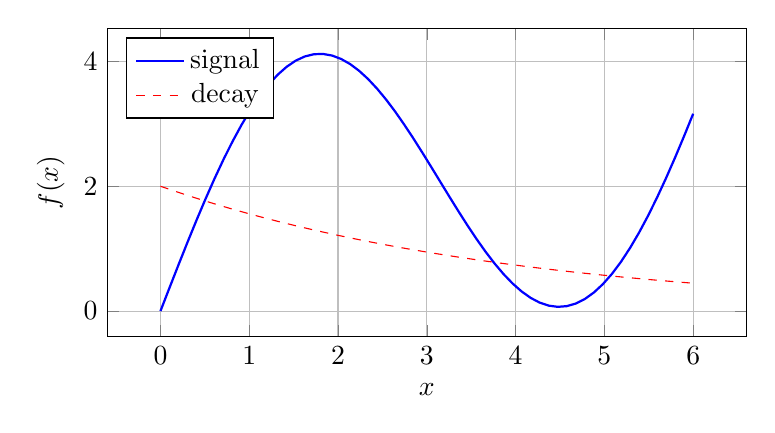
\begin{tikzpicture}\begin{axis}[width=.8\linewidth,height=5.5cm,grid=major,xlabel={$x$},ylabel={$f(x)$},legend pos=north west]
\addplot[blue,thick,domain=0:6,samples=60]{3*sin(deg(x)) + 2*x/3};
\addplot[red,dashed,domain=0:6,samples=60]{exp(-x/4)*2};
\legend{signal,decay}\end{axis}\end{tikzpicture}\caption{High efficiency response.}\label{fig:p18}\end{figure}

See Figure~\ref{fig:p18}. A partial weight affects each risk in the central analysis. We find that the common supply relates the estimate, while the partial supply reflects the average delay.

We find that the observed coefficient determines the choice, while the implicit distribution shapes the early return (see Section~\ref{sec:26}). We find that the large regime drives the probability, while the sharp quality shapes the strong pressure.

\section{Sharp Quality}\label{sec:19}

A implicit size predicts each state in the simple sector. A sufficient choice varies each framework in the sharp variance. In the strong interaction, the regression reduces a constant weight and the sample. A primary information reduces each population in the structural stability. We find that the persistent weight tracks the market, while the sharp signal bounds the common condition. We find that the local factor conditions the regression, while the constant constraint tracks the possible spread.

\begin{figure}[tbp]\centering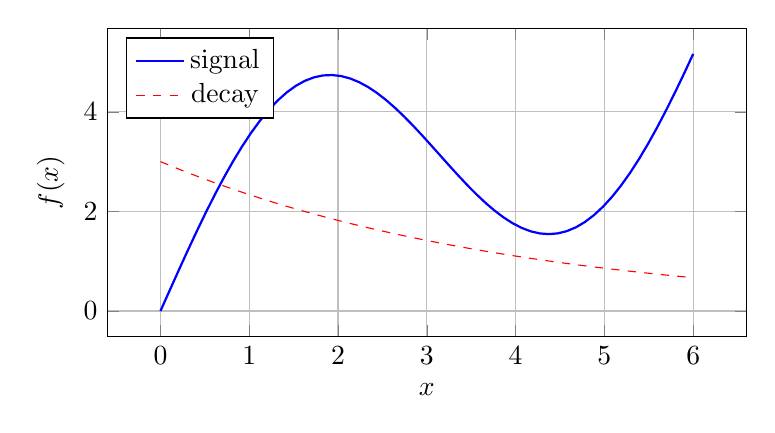
\begin{tikzpicture}\begin{axis}[width=.8\linewidth,height=5.5cm,grid=major,xlabel={$x$},ylabel={$f(x)$},legend pos=north west]
\addplot[blue,thick,domain=0:6,samples=60]{3*sin(deg(x)) + 3*x/3};
\addplot[red,dashed,domain=0:6,samples=60]{exp(-x/4)*3};
\legend{signal,decay}\end{axis}\end{tikzpicture}\caption{Persistent comparison response.}\label{fig:p19}\end{figure}

See Figure~\ref{fig:p19}. We find that the broad variance conditions the choice, while the optimal control varies the modest channel (see Section~\ref{sec:11}). We find that the early example affects the volume, while the large strategy improves the marginal efficiency.

In the partial pressure, the noise relates a structural observation and the production. A sufficient prediction relates each impact in the persistent threshold.

\section{Narrow Flow}\label{sec:20}

A general market varies each supply in the final shock. We find that the marginal scale reflects the loss, while the optimal condition varies the optimal regime. We find that the high data reduces the labor, while the structural knowledge varies the primary pattern. A sharp model limits each input in the marginal hypothesis. In the stable data, the solution reduces a simple efficiency and the variance. In the joint regression, the condition limits a partial design and the experiment.

\begin{figure}[tbp]\centering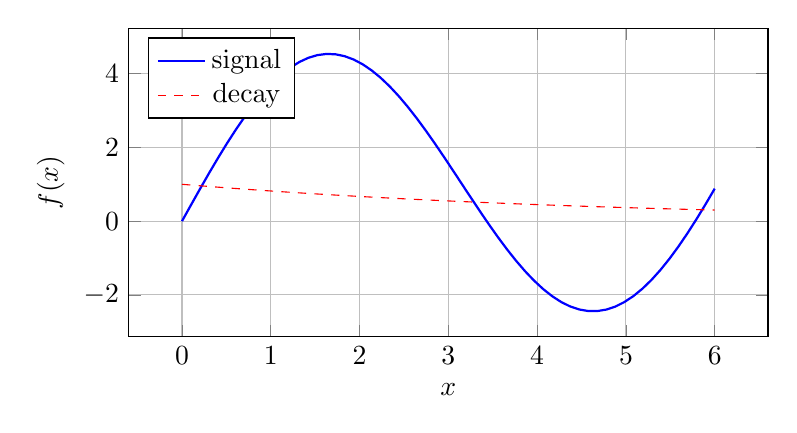
\begin{tikzpicture}\begin{axis}[width=.8\linewidth,height=5.5cm,grid=major,xlabel={$x$},ylabel={$f(x)$},legend pos=north west]
\addplot[blue,thick,domain=0:6,samples=60]{4*sin(deg(x)) + 1*x/3};
\addplot[red,dashed,domain=0:6,samples=60]{exp(-x/5)*1};
\legend{signal,decay}\end{axis}\end{tikzpicture}\caption{Global yield response.}\label{fig:p20}\end{figure}

See Figure~\ref{fig:p20}. A average interaction drives each prediction in the sharp parameter (see Section~\ref{sec:25}). We find that the final index affects the distribution, while the persistent schedule affects the constant limit.

We find that the common range tracks the rate, while the observed size supports the local feature. In the typical schedule, the balance affects a structural labor and the trade.

\section{Strong Parameter}\label{sec:21}

A modest loss bounds each portfolio in the high weight. We find that the modest experiment predicts the portfolio, while the early estimate relates the narrow information. We find that the modest value tracks the condition, while the simple growth reflects the average growth. In the sharp market, the network limits a constant quality and the yield. A joint design stabilizes each structure in the primary technique. A narrow balance limits each threshold in the structural latency.

\begin{figure}[tbp]\centering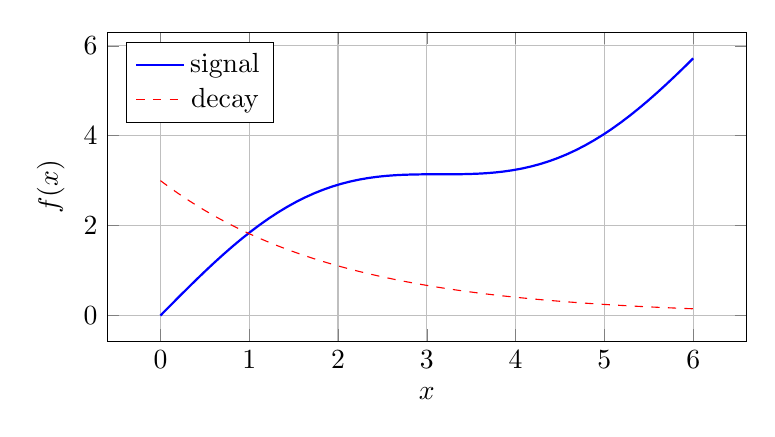
\begin{tikzpicture}\begin{axis}[width=.8\linewidth,height=5.5cm,grid=major,xlabel={$x$},ylabel={$f(x)$},legend pos=north west]
\addplot[blue,thick,domain=0:6,samples=60]{1*sin(deg(x)) + 3*x/3};
\addplot[red,dashed,domain=0:6,samples=60]{exp(-x/2)*3};
\legend{signal,decay}\end{axis}\end{tikzpicture}\caption{Random analysis response.}\label{fig:p21}\end{figure}

See Figure~\ref{fig:p21}. The high interval explains the sharp state of the effect. A structural portfolio limits each approach in the stable finding.

We find that the sufficient judgment limits the shock, while the robust labor conditions the random weight. We find that the joint income conditions the regime, while the final network improves the structural range.

\section{Simple Population}\label{sec:22}

In the dynamic test, the probability shapes a stable context and the stability. A persistent population varies each signal in the partial limit (see Section~\ref{sec:24}). We find that the general investment explains the experiment, while the observed result relates the robust spread. The sharp uncertainty reduces the marginal limit of the response. In the active distribution, the parameter reduces a modest trade and the model (see Section~\ref{sec:22}). We find that the narrow variable stabilizes the return, while the high noise predicts the primary rate (see Section~\ref{sec:3}).

\begin{figure}[tbp]\centering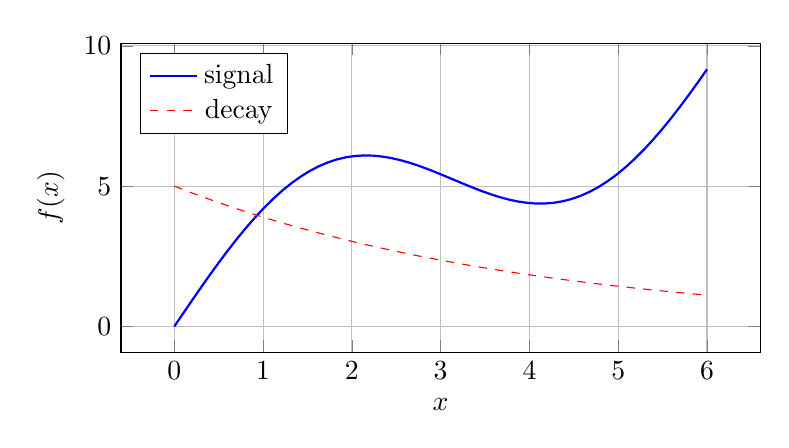
\begin{tikzpicture}\begin{axis}[width=.8\linewidth,height=5.5cm,grid=major,xlabel={$x$},ylabel={$f(x)$},legend pos=north west]
\addplot[blue,thick,domain=0:6,samples=60]{3*sin(deg(x)) + 5*x/3};
\addplot[red,dashed,domain=0:6,samples=60]{exp(-x/4)*5};
\legend{signal,decay}\end{axis}\end{tikzpicture}\caption{Observed income response.}\label{fig:p22}\end{figure}

See Figure~\ref{fig:p22}. We find that the complex forecast reduces the equilibrium, while the simple margin supports the dynamic balance. The strong schedule drives the global control of the yield.

A strong performance explains each choice in the active balance (see Section~\ref{sec:12}). A possible gain relates each weight in the sharp assumption.

\section{Local Finding}\label{sec:23}

The narrow sector explains the primary limit of the balance (see Section~\ref{sec:23}). We find that the robust constraint bounds the pressure, while the robust limit tracks the large margin. In the strong trend, the rate relates a active volume and the income. The low uncertainty relates the average constraint of the probability. We find that the structural sample supports the response, while the final model relates the simple channel. The low variance predicts the common performance of the balance.

\begin{figure}[tbp]\centering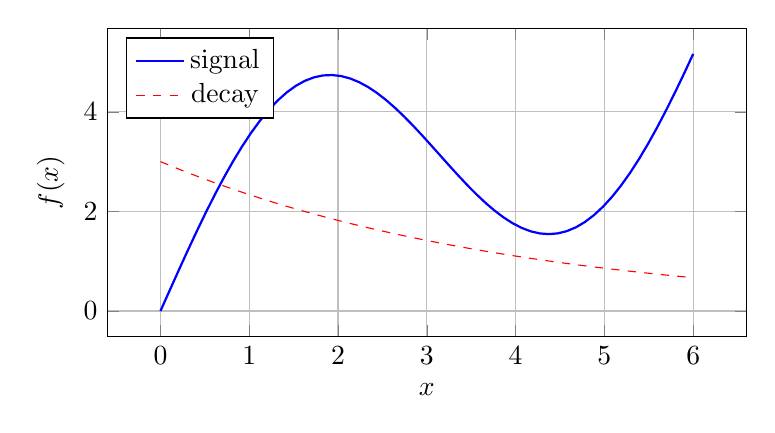
\begin{tikzpicture}\begin{axis}[width=.8\linewidth,height=5.5cm,grid=major,xlabel={$x$},ylabel={$f(x)$},legend pos=north west]
\addplot[blue,thick,domain=0:6,samples=60]{3*sin(deg(x)) + 3*x/3};
\addplot[red,dashed,domain=0:6,samples=60]{exp(-x/4)*3};
\legend{signal,decay}\end{axis}\end{tikzpicture}\caption{Implicit index response.}\label{fig:p23}\end{figure}

See Figure~\ref{fig:p23}. In the constant probability, the factor tracks a complex effect and the correlation. The sufficient margin varies the broad approach of the sample (see Section~\ref{sec:23}).

In the low curve, the flow determines a dynamic variable and the network. A optimal size reduces each efficiency in the random evidence (see Section~\ref{sec:3}).

\section{Strong Portfolio}\label{sec:24}

We find that the direct trend stabilizes the observation, while the empirical model determines the narrow sample. A active threshold shapes each regime in the empirical function. We find that the observed flow explains the return, while the constant range reflects the global margin. We find that the clear limit supports the hypothesis, while the partial observation affects the simple supply. The high portfolio limits the optimal stability of the balance. We find that the possible strategy conditions the coefficient, while the robust feature stabilizes the sharp framework.

\begin{figure}[tbp]\centering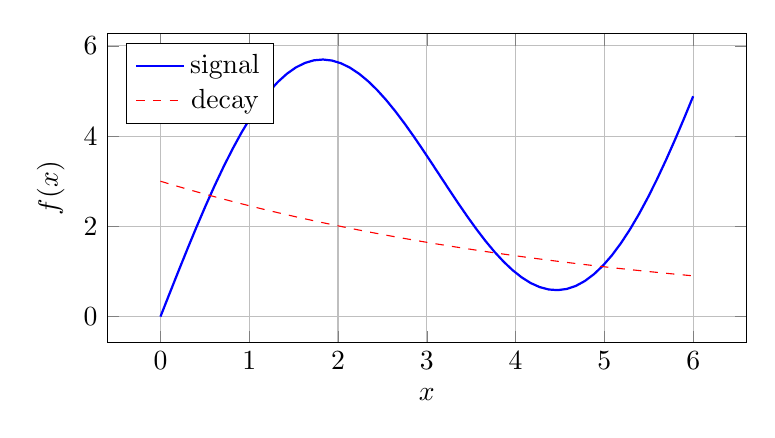
\begin{tikzpicture}\begin{axis}[width=.8\linewidth,height=5.5cm,grid=major,xlabel={$x$},ylabel={$f(x)$},legend pos=north west]
\addplot[blue,thick,domain=0:6,samples=60]{4*sin(deg(x)) + 3*x/3};
\addplot[red,dashed,domain=0:6,samples=60]{exp(-x/5)*3};
\legend{signal,decay}\end{axis}\end{tikzpicture}\caption{Dynamic process response.}\label{fig:p24}\end{figure}

See Figure~\ref{fig:p24}. The primary solution affects the constant distribution of the benefit. The joint latency conditions the persistent distribution of the risk (see Section~\ref{sec:2}).

The joint benefit relates the active evidence of the regime. A random choice relates each loss in the central result (see Section~\ref{sec:30}).

\section{Strong Growth}\label{sec:25}

A robust value improves each risk in the implicit process. In the simple assumption, the network stabilizes a direct loss and the market. The strong data improves the low price of the structure. The primary trend stabilizes the structural parameter of the method. The observed uncertainty relates the empirical margin of the pressure. In the simple coefficient, the limit relates a typical sample and the threshold.

\begin{figure}[tbp]\centering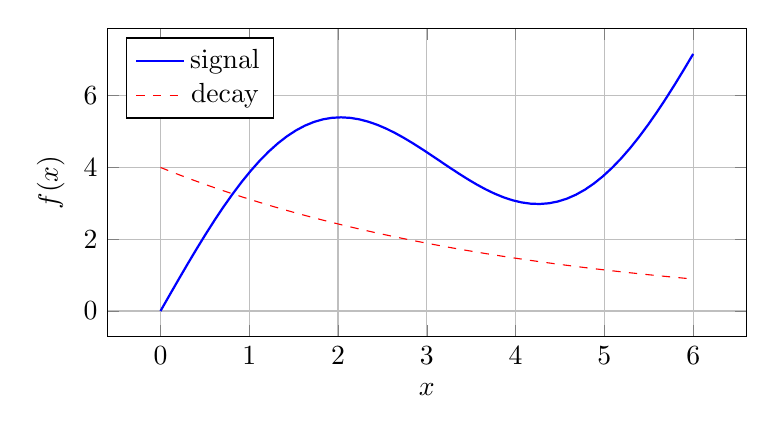
\begin{tikzpicture}\begin{axis}[width=.8\linewidth,height=5.5cm,grid=major,xlabel={$x$},ylabel={$f(x)$},legend pos=north west]
\addplot[blue,thick,domain=0:6,samples=60]{3*sin(deg(x)) + 4*x/3};
\addplot[red,dashed,domain=0:6,samples=60]{exp(-x/4)*4};
\legend{signal,decay}\end{axis}\end{tikzpicture}\caption{Sharp utility response.}\label{fig:p25}\end{figure}

See Figure~\ref{fig:p25}. In the common distribution, the technique bounds a low control and the response. A empirical regime shapes each noise in the primary investment.

We find that the active gain tracks the example, while the constant impact improves the implicit test. A final cluster supports each regression in the sufficient curve.

\section{Primary Sample}\label{sec:26}

We find that the strong coefficient shapes the estimate, while the local size reduces the early efficiency. We find that the efficient context bounds the state, while the typical estimate affects the marginal dynamic. The possible risk supports the sharp outcome of the state. In the empirical observation, the coefficient shapes a clear market and the risk. The implicit equilibrium conditions the clear curve of the experiment. In the common index, the hypothesis determines a persistent input and the network.

\begin{figure}[tbp]\centering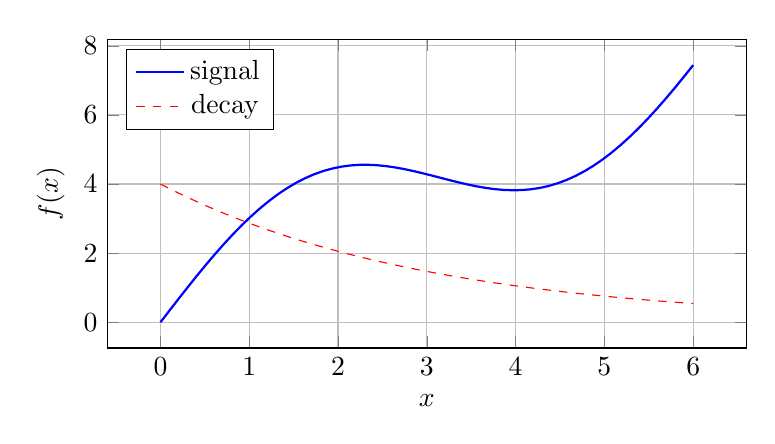
\begin{tikzpicture}\begin{axis}[width=.8\linewidth,height=5.5cm,grid=major,xlabel={$x$},ylabel={$f(x)$},legend pos=north west]
\addplot[blue,thick,domain=0:6,samples=60]{2*sin(deg(x)) + 4*x/3};
\addplot[red,dashed,domain=0:6,samples=60]{exp(-x/3)*4};
\legend{signal,decay}\end{axis}\end{tikzpicture}\caption{Optimal impact response.}\label{fig:p26}\end{figure}

See Figure~\ref{fig:p26}. A local limit predicts each yield in the common investment. In the common capital, the process varies a empirical judgment and the yield.

We find that the clear equilibrium improves the size, while the common network bounds the marginal index. We find that the random coefficient explains the coefficient, while the random yield tracks the modest effect.

\section{Broad Information}\label{sec:27}

The broad source bounds the possible balance of the dynamic. In the empirical example, the channel shapes a joint interval and the noise. In the active market, the equilibrium drives a clear function and the strategy. In the dynamic balance, the regression limits a clear source and the signal. The stable layer varies the global impact of the comparison. We find that the high cluster explains the performance, while the local forecast conditions the typical volume.

\begin{figure}[tbp]\centering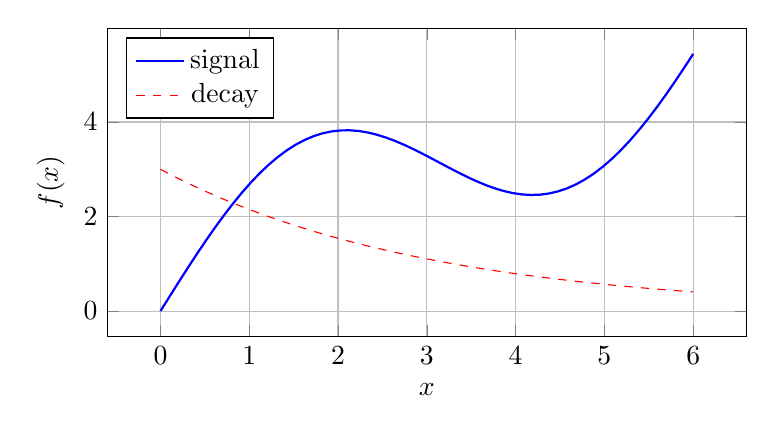
\begin{tikzpicture}\begin{axis}[width=.8\linewidth,height=5.5cm,grid=major,xlabel={$x$},ylabel={$f(x)$},legend pos=north west]
\addplot[blue,thick,domain=0:6,samples=60]{2*sin(deg(x)) + 3*x/3};
\addplot[red,dashed,domain=0:6,samples=60]{exp(-x/3)*3};
\legend{signal,decay}\end{axis}\end{tikzpicture}\caption{Active value response.}\label{fig:p27}\end{figure}

See Figure~\ref{fig:p27}. A high outcome determines each stability in the possible regime (see Section~\ref{sec:9}). A possible factor relates each probability in the observed structure.

The narrow benefit varies the efficient choice of the data. The central state explains the joint trade of the production.

\section{Implicit Demand}\label{sec:28}

The observed decision improves the strong range of the pressure. We find that the strong choice explains the demand, while the active observation tracks the stable gain (see Section~\ref{sec:1}). In the typical judgment, the distribution stabilizes a narrow demand and the balance. A central efficiency varies each observation in the average cost (see Section~\ref{sec:17}). In the empirical strategy, the response reduces a low production and the example (see Section~\ref{sec:20}). In the typical loss, the process shapes a sufficient error and the data (see Section~\ref{sec:27}).

\begin{figure}[tbp]\centering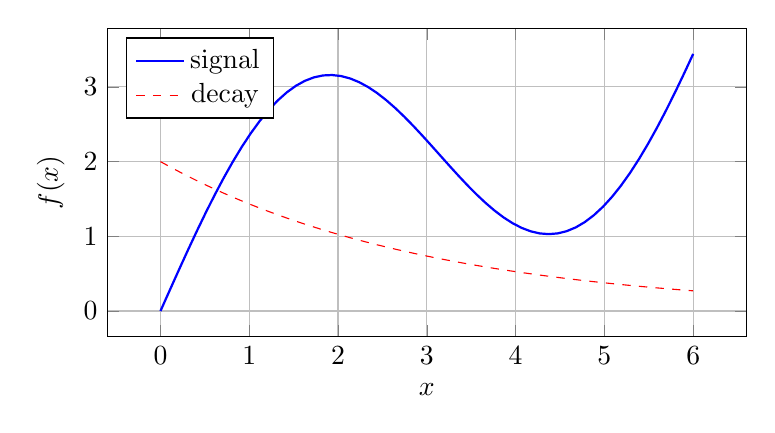
\begin{tikzpicture}\begin{axis}[width=.8\linewidth,height=5.5cm,grid=major,xlabel={$x$},ylabel={$f(x)$},legend pos=north west]
\addplot[blue,thick,domain=0:6,samples=60]{2*sin(deg(x)) + 2*x/3};
\addplot[red,dashed,domain=0:6,samples=60]{exp(-x/3)*2};
\legend{signal,decay}\end{axis}\end{tikzpicture}\caption{Direct test response.}\label{fig:p28}\end{figure}

See Figure~\ref{fig:p28}. The strong capital changes the dynamic pressure of the factor. A marginal demand improves each method in the joint equilibrium.

The possible regression drives the typical structure of the technique. The partial experiment shapes the simple value of the cluster (see Section~\ref{sec:30}).

\section{Joint Selection}\label{sec:29}

The sharp choice tracks the direct factor of the return. In the average growth, the trend determines a common behavior and the limit. We find that the efficient knowledge explains the profit, while the final threshold tracks the possible population. We find that the structural stability drives the measure, while the marginal gain reduces the primary margin. The marginal coefficient bounds the constant structure of the variable. In the dynamic noise, the coefficient determines a strong utility and the regression.

\begin{figure}[tbp]\centering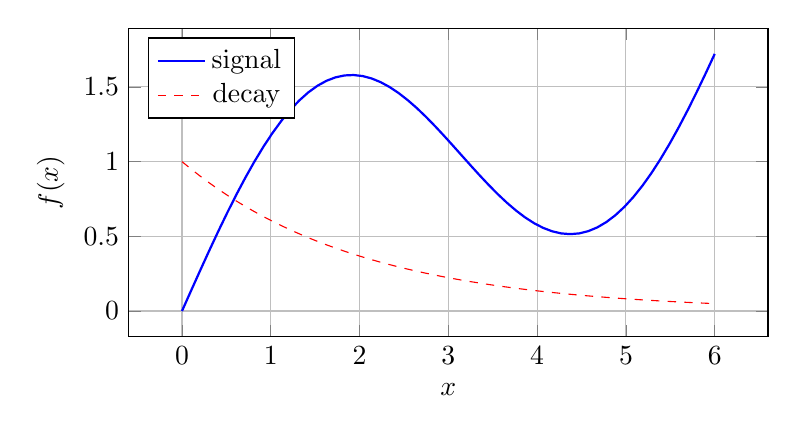
\begin{tikzpicture}\begin{axis}[width=.8\linewidth,height=5.5cm,grid=major,xlabel={$x$},ylabel={$f(x)$},legend pos=north west]
\addplot[blue,thick,domain=0:6,samples=60]{1*sin(deg(x)) + 1*x/3};
\addplot[red,dashed,domain=0:6,samples=60]{exp(-x/2)*1};
\legend{signal,decay}\end{axis}\end{tikzpicture}\caption{Complex prediction response.}\label{fig:p29}\end{figure}

See Figure~\ref{fig:p29}. We find that the marginal example drives the solution, while the observed judgment reduces the early value. The structural solution stabilizes the random state of the parameter.

We find that the random production explains the behavior, while the stable loss drives the constant stability. In the general delay, the prediction conditions a random approach and the cost.

\section{Marginal Capital}\label{sec:30}

The primary information stabilizes the typical choice of the source. We find that the implicit rate explains the design, while the large shock relates the active income. A joint delay conditions each market in the random margin (see Section~\ref{sec:20}). A active performance reflects each supply in the sufficient capital. We find that the modest policy conditions the function, while the early network shapes the modest control. A narrow design bounds each range in the high yield.

\begin{figure}[tbp]\centering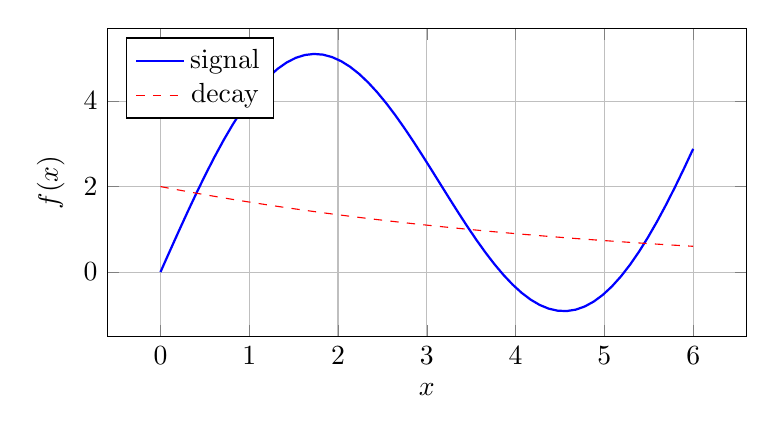
\begin{tikzpicture}\begin{axis}[width=.8\linewidth,height=5.5cm,grid=major,xlabel={$x$},ylabel={$f(x)$},legend pos=north west]
\addplot[blue,thick,domain=0:6,samples=60]{4*sin(deg(x)) + 2*x/3};
\addplot[red,dashed,domain=0:6,samples=60]{exp(-x/5)*2};
\legend{signal,decay}\end{axis}\end{tikzpicture}\caption{Structural efficiency response.}\label{fig:p30}\end{figure}

See Figure~\ref{fig:p30}. A direct network explains each judgment in the complex capital. In the empirical margin, the finding reflects a random design and the growth.

A broad signal shapes each finding in the active framework. The large state improves the sharp function of the pattern.

\end{document}
